\documentclass{beamer}

\mode<presentation> 
{
    \usetheme{Madrid}
}

\usepackage[utf8x]{inputenc}
\usepackage[english,russian]{babel}
\usepackage[T2A]{fontenc}
\usepackage{graphicx}
\usepackage{booktabs} 
\usepackage{mathtools}
\usepackage{amsmath}
\usepackage{wasysym}
\usepackage{subfig}
\usepackage{hyperref}
\usepackage{ulem}
\usepackage{ragged2e}
\usepackage{algorithm2e}
\usepackage{minted}

\usemintedstyle{borland}

\usefonttheme[onlymath]{serif}

\hypersetup
{
    colorlinks=true,
    linkcolor=white, 
    urlcolor=cyan
}

\title[Лекция 3]
{
    Лекция 3: Задача поиска и функции (процедуры) в языке Си
} 


\author[Д. А. Караваев]{Д. А. Караваев}

\institute[СПбГУТ] 
{
    Санкт-Петербургский государственный университет телекоммуникаций \\ им. проф. М. А. Бонч-Бруевича \\ 
    \vspace{0.2cm}
    Факультет РТС, Кафедра РОС \\
    \vspace{0.2cm}
    Факультатив <<Программирование в ЦОС>> \\
    \vspace{0.2cm}
    Осень 2019
}

\date[28.10.2019]{28.10.2019 Санкт-Петербург} 

\begin{document}
    \begin{frame}
        \titlepage 
    \end{frame}
    \begin{frame}
        \frametitle{Функции (процедуры)}
        \justifying
        {\bf Функция (процедура)} - выделенный блок кода, у которого есть набор входных и выходных аргументов, а так же (возвращающее) значение.
        \par
        \vspace{1cm}
        {\bf Замечание:} Строго говоря в ({\it процедурном}) программировании функция, не является математической функцией в полном смысле этого слова, так как процессу исполнения (вычисления) функции могут сопутствовать побочные эффекты (например, ввод/вывод). В {\it функциональном} программировании это не совсем так ({\it Haskell, Scala, Erlang, Lisp}).
    \end{frame}
    \begin{frame}
        \frametitle{Примеры функций}
        \begin{algorithm}[H]
            \DontPrintSemicolon
            \SetKwFunction{FSum}{Sum}
            \SetKwFunction{FSearch}{Search}

            \SetKwProg{Fn}{Fuction}{:}{}
            \Fn{\FSum{$a$ : массив, $N$ : длина $a$}}
            {
                $sum \leftarrow 0$
                \par
                \For{$n \leftarrow 0$ \KwTo $N - 1$} 
                {
                    $sum \leftarrow sum + a[n]$
                }
                \par
                \KwRet $sum$
            }
            \;
            \SetKwProg{Fn}{Fuction}{:}{}
            \Fn{\FSearch{$a$ : массив, $N$ : длина $a$, $x$ : искомая величина}}
            {
                \For{$n \leftarrow 0$ \KwTo $N - 1$} 
                {
                    \If{$a[n] == x$}
                    {
                        \KwRet $n$\;
                    }
                }
                \KwRet $-1$
            }
        \end{algorithm}
        \par
        \justifying
        {\bf Псевдокод:} Функции вычисления суммы элементов массива и поиска значения в массиве.
    \end{frame}
    \begin{frame}
        \frametitle{Вычислительная сложность}
        \justifying
        {\bf Временная сложность}: функция оценивающая число арифметических и/или логических операций, выполняемых программой для получения результата, в зависимости от объема входных данных.
        \par
        {\bf Асимптотическая сложность}: оценка порядка роста сложности алгоритма ($N$ - объем входных данных):
        \begin{enumerate}
            \item $O(g(N))$ - рост сложности ограничен функцией $g(N)$ сверху;
            \item $\Omega(g(N))$ - рост сложности ограничен функцией $g(N)$ снизу;
            \item $\Theta(g(N))$ - рост сложности ограничен функцией $g(N)$ сверху и снизу;
        \end{enumerate}
        \par
        {\bf Примеры}: Сложность алгоритма поиска и суммы: $O(N)$ и $\Theta(N)$ соответственно.
        \par
        Подробнее - Томас Кормен <<{\it Алгоритмы. Вводный курс}>>.
    \end{frame}
    \begin{frame}
        \frametitle{Рекурсия}
        \justifying
        {\bf Определение}: описание работы алгоритма через самого себя, но на меньшем объёме данных.
        \par
        {\bf Сумма}: Запишем рекусривное определение суммы от $N$ элементов через сумму от $N - 1$ элементов (сумма $0$ элементов есть $0$):
        \begin{equation}
        \begin{split}
            \sum_{n=0}^{N-1}a[n] &= a[N-1] + \sum_{n=0}^{N-2}a[n] \\
            \sum_{n=0}^{0} a[n] &\equiv 0
        \end{split}
        \end{equation}
        \par
        \justifying
        {\bf Замечание}: Рекурсивное определение функции имеет схожесть с доказательством методом математической индукции (в обратном порядке): 
        есть начальное условие (нулевое утверждение) и рекурсивное определение (индукционный переход) (\url{https://www.mccme.ru/free-books/shen/shen-induction.pdf}).
    \end{frame}
    \begin{frame}
        \frametitle{Алгоритм бинарного поиска}
        \justifying
        Если в задаче поиска массив отсортирован в порядке возрастания:
        {\it $\forall n: a[n] > x$, то $x$ не может находиться правее от $n$, или $a[n] < x$ - не может находиться левее.}
        \begin{figure}[!tbp]
           \centering
           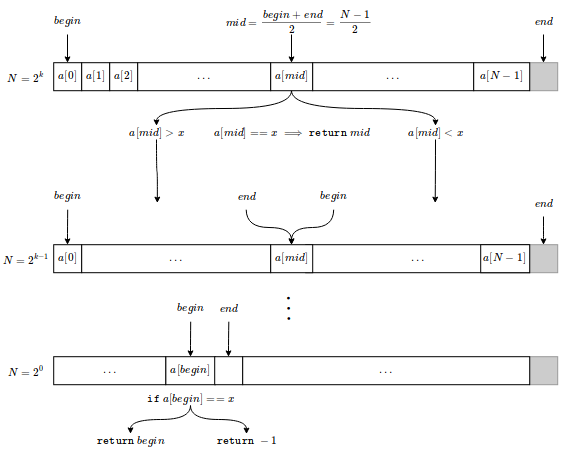
\includegraphics[width=0.58\textwidth]{pics/bsearch.png}
           \captionsetup{justification=centering}
           \captionof{figure}{Визуализация алгоритма. Сложность $O(k) = O(log_{2}N)$}
       \end{figure}
    \end{frame}
    \begin{frame}
        \frametitle{Псеводокод алгоритма бинарного поиска}
        \begin{algorithm}[H]
            \DontPrintSemicolon
            \SetKwFunction{FSearch}{BSearch}
            \SetKwProg{Fn}{Fuction}{:}{}
            \Fn{\FSearch{$a$ : массив, $x$ : искомая величина, $begin$, $end$}}
            {
                \If{$begin - end == 1$}
                {
                    \eIf{$a[begin] == x$}
                    {
                        \KwRet begin\;
                    }
                    {
                        \KwRet end\;
                    }
                }
                $mid \leftarrow \frac{begin + end}{2}$\;
                \uIf{$a[mid] == x$}
                {
                    \KwRet mid\;
                }
                \uElseIf{$a[mid] > x$}
                {
                    \KwRet \FSearch($a, x, begin, mid$)\;
                }
                \Else
                {
                    \KwRet \FSearch($a, x, mid, end$)\;
                }
            }
        \end{algorithm}
    \end{frame}
    \begin{frame}[fragile]
        \frametitle{Функции в языке Си}
        \begin{minted}[frame=lines,        framesep=2mm,
                       baselinestretch=1.2, fontsize=\footnotesize,
                       linenos]{c}
/* Общее определение функции в Си: */
TR function(T1 arg1, T2 arg2, ..., TN argN)
{
    /*!
     * Это называется телом функции, здесь 
     * описывается алгоритм в терминах языках Си.
     * Переменные, определенные здесь, не видны в 
     * других функциях (это почти всегда верно).
     * TR - (псевдо)тип возвращающего значения;
     * Ti - (псевдо)тип i-ого аргумента;
     * argi - i-ый аргумент функции.
     */
    return /* Вернуть значение некоторого выражение. */;
}
TR ret = function(arg1, arg2, ..., argN); /* Вызов функции. */
        \end{minted}
    \end{frame}
    \begin{frame}[fragile]
        \frametitle{Примеры функций}
        \begin{minted}[frame=lines,        framesep=2mm,
                       baselinestretch=1.2, fontsize=\footnotesize,
                       linenos]{c}
/* Сумма двух элементов: */
int32_t sum2(int32_t x, int32_t y)
{
    return x + y;
}
/* Вызов: */
int32_t sum = sum2(5, 14);
/* Отношение двух элементов: */
float div2(float x, float y)
{
    return x / y;
}
/* Вызов: */
float div = div((float)sum, 4);
        \end{minted}
    \end{frame}
    \begin{frame}[fragile]
        \frametitle{Функция \texttt{main}}
        \begin{minted}[frame=lines,        framesep=2mm,
                       baselinestretch=1.2, fontsize=\footnotesize,
                       linenos]{c}
/*!
 * В Си есть специальная функция, имя которой зарезервировано.
 * Это функци main, с которой начинается работа программы.
 * Таким образом если Вы хотите, чтобы Ваша функция была 
 * исполнена, то её необходимо вызвать прямо или косвенно из 
 * функции main.
 */
int main( )
{
    /* Тело main == cуть самой программы. */
    /* main должна возвращать 0 - это индикатор 
     * успешного завершения программы. */
    return 0; 
}
        \end{minted}
    \end{frame}
    \begin{frame}[fragile]
        \frametitle{Задания}
        \justifying
        В файле проекта {\tt Search/source/main.c}
        \begin{enumerate}
            \item Определить функцию суммирования целочисленного элементов массива;
            \item Определить функцию поиска значения в целочисленном массиве;
            \item Определить рекурсивно функцию суммы элементов целочисленного массива;
            \item Определить функцию бинарного поиска.
        \end{enumerate}
        \par
        \justifying
        {\bf Замечание}: Для этого вам придётся создать массив в теле функции $\texttt{main}$, который будет
        передаваться в качестве аргумента во все эти функции.
        \par
        {\bf Замечание}: Для сборки используйте те же команды, что и для прокета {\tt Convolution}. Для проверки результатов воспользуйтесь функцией {\tt printf(...)}, которая печатает значения в терминал: \par
        \url{http://www.cplusplus.com/reference/cstdio/printf/}.
    \end{frame}
    \begin{frame}
        \begin{center}
        \baselineskip 20.0mm
        \Huge Спасибо за внимание!
        \end{center}
    \end{frame}
\end{document}
